\documentclass[10pt]{article}
\usepackage[paperwidth=24cm, paperheight=24cm, top=1.3cm, bottom=1.3cm, left=1.6cm, right=1.6cm]{geometry}
\usepackage{fontspec}
\usepackage{xcolor}
\usepackage{graphicx}
\usepackage{multicol}

% Estética de Vinil Anos 70 (Papel Pólen Envelhecido, Tinta Sépia/Café e Terracota)
\definecolor{vinylpaper}{HTML}{F3EAD8}
\definecolor{vinylink}{HTML}{1E1610}
\definecolor{vinylrust}{HTML}{8C3B2B}
\definecolor{vinylochre}{HTML}{B57B3A}
\definecolor{vinylmuted}{HTML}{5E4D3B}
\definecolor{vinyldark}{HTML}{140F0B}

\setmainfont{Baskerville}[
  Ligatures=TeX,
  Scale=1.0
]
\setsansfont{Helvetica Neue}[
  Scale=0.92
]
\setmonofont{American Typewriter}[
  Scale=0.88
]

\setlength{\parindent}{0pt}
\setlength{\parskip}{3pt}
\setlength{\columnsep}{1.0cm}
\pagestyle{empty}

\newcommand{\pageheader}[1]{%
  \noindent{\texttt{\scriptsize\color{vinylmuted} GRAVETOS NO ESCURO — ENCARTE DE VINIL (33 1/3 RPM)}\hfill\texttt{\scriptsize\color{vinylmuted} #1}}\par
  \vspace{-0.18cm}
  \noindent{\color{vinylochre}\rule{\textwidth}{0.5pt}}\par
  \vspace{0.12cm}
}

\newcommand{\trackheader}[6]{%
  \vspace{0.18cm}
  \noindent{\color{vinylrust}\rule{\linewidth}{0.9pt}}\par\vspace{0.05cm}
  \noindent{\normalsize\bfseries\color{vinylrust} #1. #2}\hfill{\texttt{\scriptsize\color{vinylmuted} LADO #3 $\cdot$ #5 BPM $\cdot$ #6}}\par
  \vspace{0.02cm}
  \noindent{\texttt{\scriptsize\color{vinylochre} ESTILO: #4}}\par
  \vspace{0.05cm}
}

\newcommand{\linernote}[1]{%
  \noindent{\itshape\footnotesize\color{vinylmuted} ``#1''}\par
  \vspace{0.10cm}
}

\begin{document}

% ============================================================================
% PÁGINA 1: CAPA DO ENCARTE (ARTE DE CAPA EM ALTA RESOLUÇÃO)
% ============================================================================
\pagecolor{vinyldark}
\color{vinylpaper}
\begin{center}
  \vspace*{0.2cm}
  \setlength{\fboxsep}{2pt}
  \setlength{\fboxrule}{1.2pt}
  \fcolorbox{vinylochre}{vinyldark}{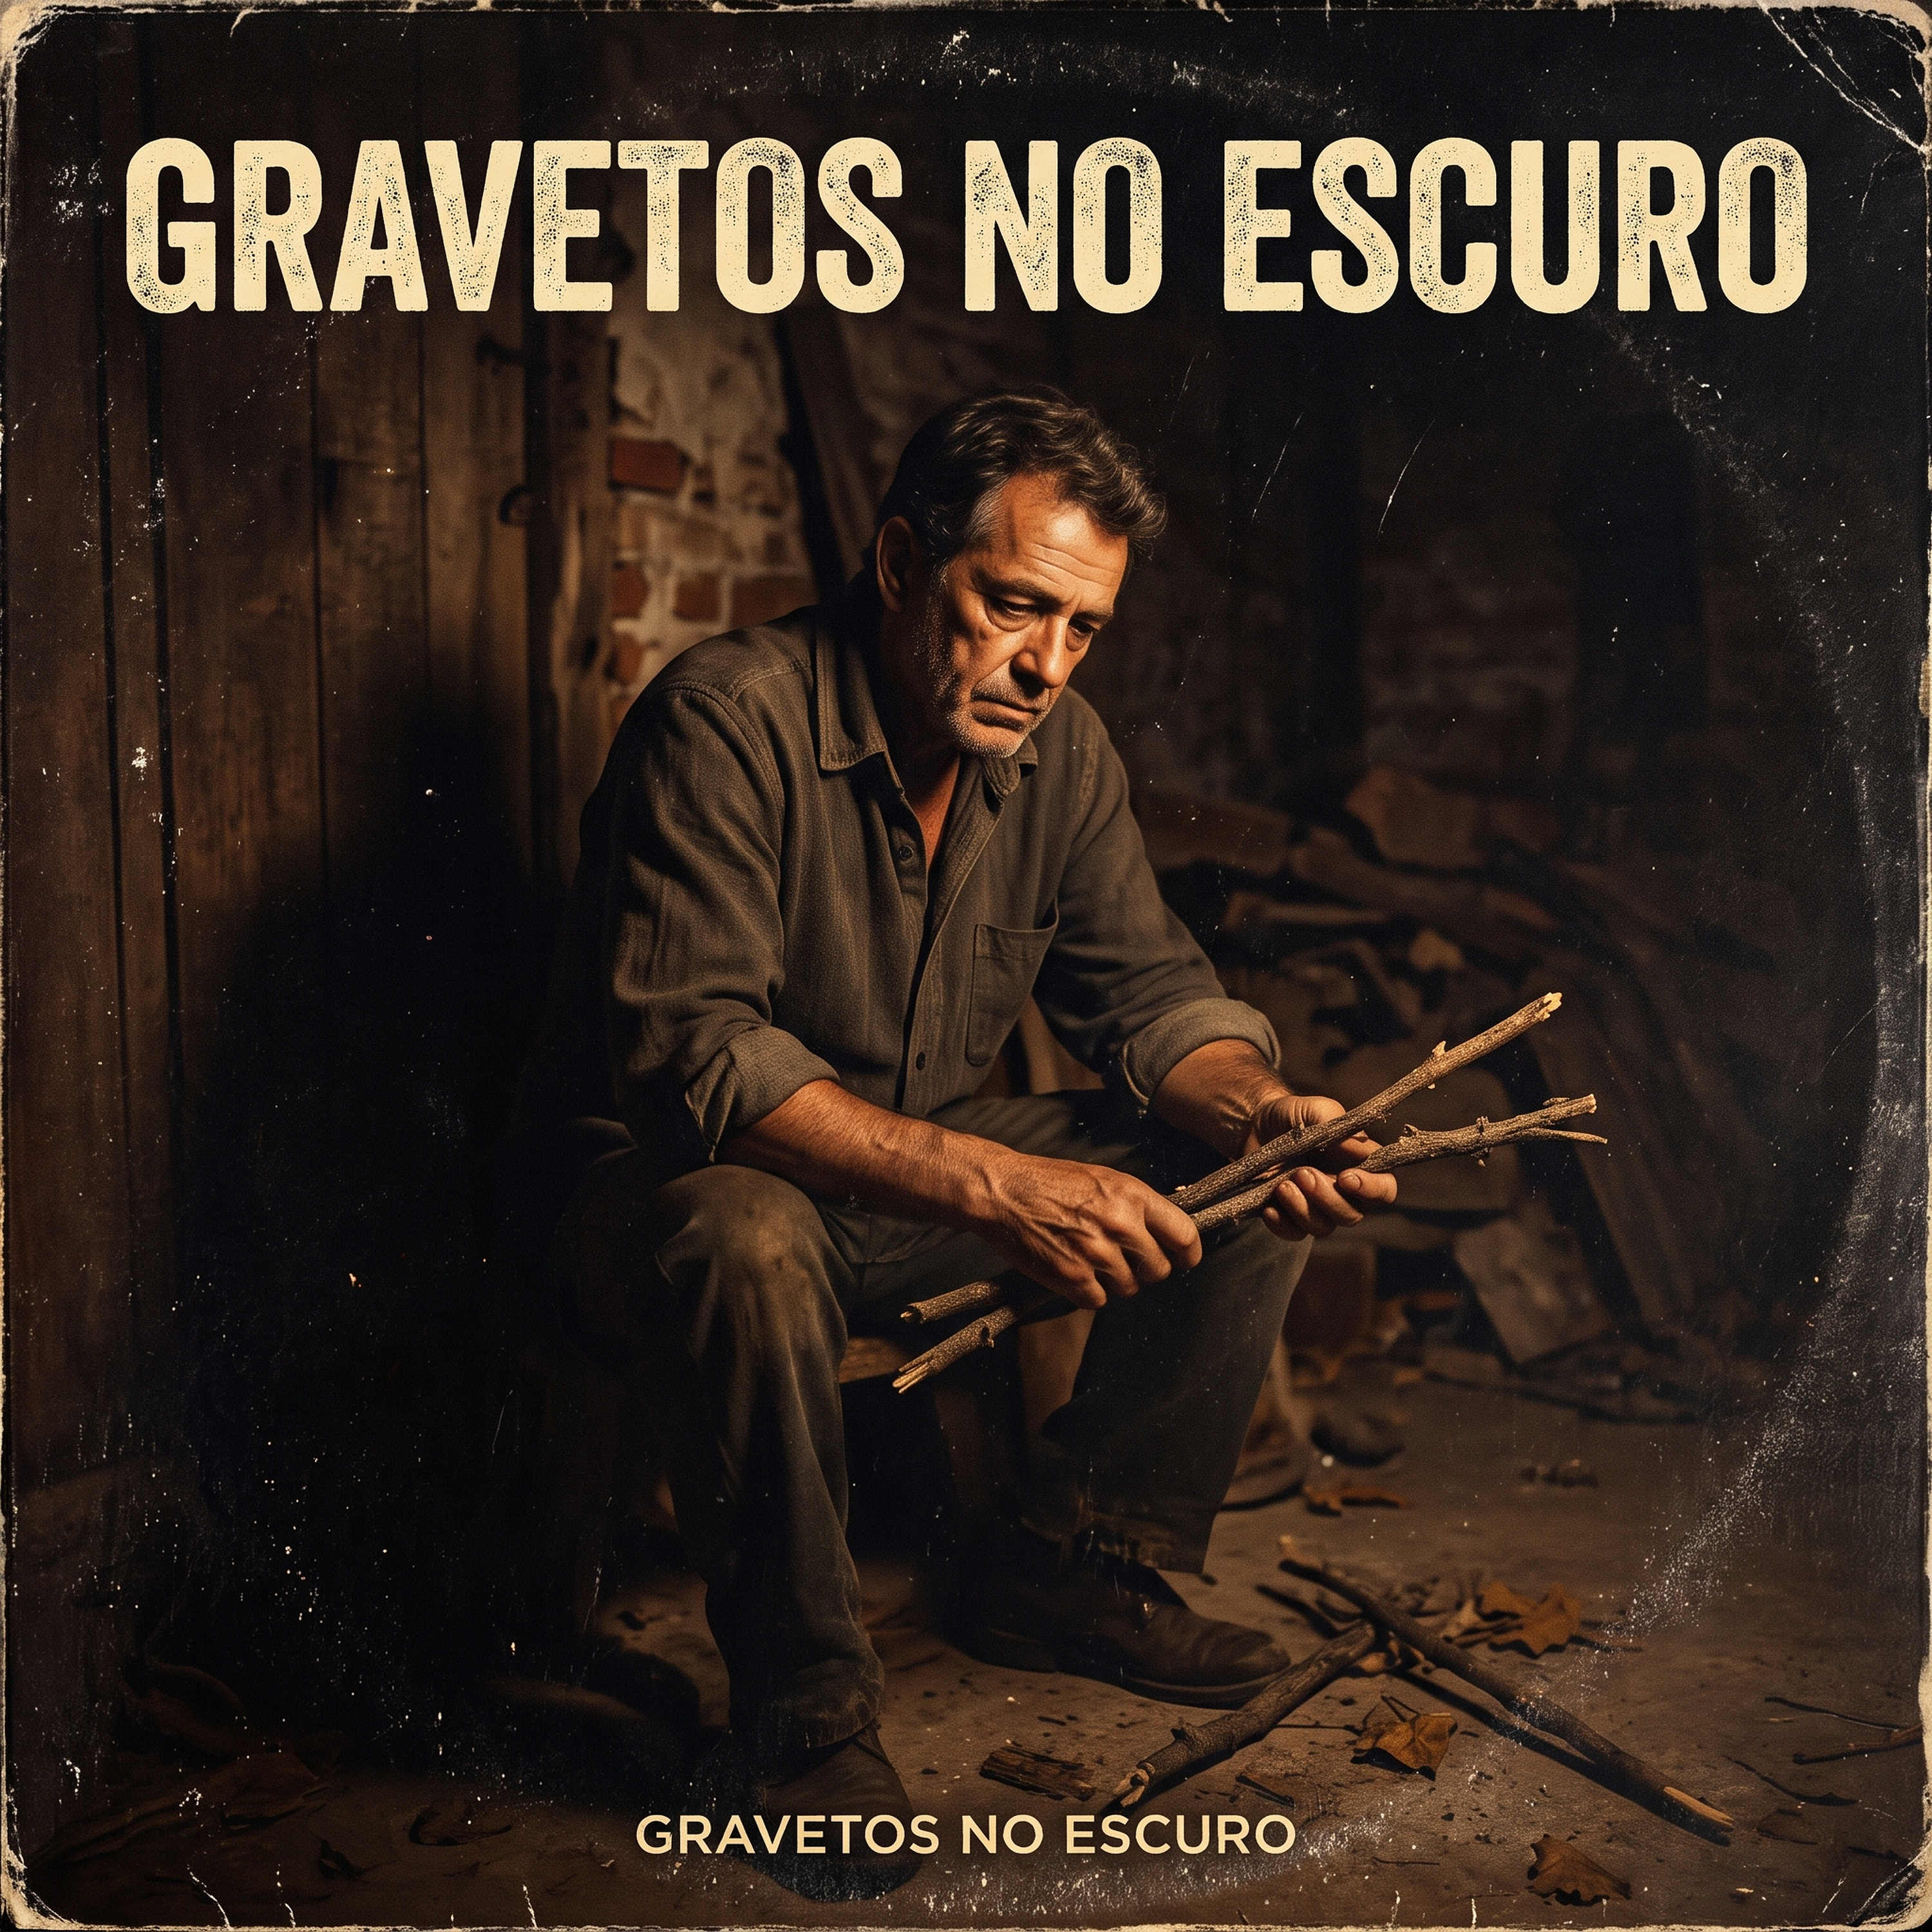
\includegraphics[width=19.4cm, height=19.4cm]{cover-3000x3000.jpg}}\par
  \vspace{0.35cm}
  {\texttt{\footnotesize\color{vinylpaper} ENCARTE MESTRE DE LETRAS E CRÔNICAS $\cdot$ EDIÇÃO DE VINIL 12 POLEGADAS}}
\end{center}
\newpage

% ============================================================================
% PÁGINA 2: CAPA INTERNA (EPÍGRAFE, FICHA TÉCNICA E TEXTO DE CONTRACAPA)
% ============================================================================
\pagecolor{vinylpaper}
\color{vinylink}

\pageheader{CAPA INTERNA \& CONTRACAPA}

\begin{center}
  {\color{vinylrust}\rule{\textwidth}{1.6pt}}\vspace{0.15cm}

  {\Huge\bfseries\color{vinylink} GRAVETOS NO ESCURO}\par
  \vspace{0.08cm}
  {\texttt{\small\color{vinylrust} LP CONCEITUAL — 9 FAIXAS (26:41) $\cdot$ LADO A \& LADO B}}\par
  \vspace{0.08cm}
  {\color{vinylrust}\rule{\textwidth}{0.6pt}}
\end{center}

\vspace{0.2cm}

\begin{center}
  \begin{minipage}{0.88\textwidth}
    \begin{center}
      {\texttt{\scriptsize\color{vinylochre} — EPÍGRAFE (CAPA INTERNA) —}}\par\vspace{0.1cm}
      {\large\itshape\color{vinylink}
      ``Não pedi licença para entrar na sala, nem recibo pelo que perdi no caminho. Juntei o que deu: três gravetos, duas âncoras no olhar e um bando na memória. Enquanto houver lenha e compasso, o escuro é só parte da estrada.''}
    \end{center}
  \end{minipage}
\end{center}

\vspace{0.25cm}
\noindent{\color{vinylochre}\rule{\textwidth}{0.6pt}}
\vspace{0.2cm}

\begin{multicols}{2}
  \noindent{\large\bfseries\color{vinylrust} TEXTO DE CONTRACAPA}\par\vspace{0.12cm}

  Há solidões que visitam; há outras que fundam a casa. Este disco nasceu no escuro de um quarto onde o relógio pesa mais que o ar, feito por quem aprendeu cedo a erguer abrigo com o que sobrou no chão.\par\vspace{0.15cm}

  No \textbf{Lado A}, o ferro frio: a infância rala, a armadura cínica da rua, o salão onde não fomos chamados, a vitrine impagável e o silêncio brutal de ver quem se ama partir sem sair do lugar. Aqui não há enfeite — o ritmo bate seco porque a dor também tem compasso.\par\vspace{0.15cm}

  Mas ninguém junta gravetos por vocação ao frio; junta-se porque a madeira seca ainda guarda fogo. Quando o disco vira para o \textbf{Lado B}, entram o passo pequeno na sala, a memória viva da mesa dividida e o suor da cozinha batucando contra o isolamento. Não é promessa de cura mágica nem final de vitrine. É o relato de quem segue de sentinela, sabendo distinguir o peso de uma tumba da travessia de um túnel.

  \columnbreak

  \noindent{\large\bfseries\color{vinylrust} FICHA TÉCNICA E ÍNDICE}\par\vspace{0.12cm}

  \noindent\texttt{\footnotesize\color{vinylmuted} FORMATO:} LP Conceitual (9 Faixas $\cdot$ 26 min 41 seg)\\
  \texttt{\footnotesize\color{vinylmuted} GÊNERO:} MPB / Samba-Canção / Samba-Rock-Groove\\
  \texttt{\footnotesize\color{vinylmuted} MASTERIZAÇÃO:} -14 LUFS / -1.5 dBTP (24-bit / 44.1kHz)\\
  \texttt{\footnotesize\color{vinylmuted} LICENÇA:} Creative Commons CC BY-SA 4.0

  \vspace{0.2cm}
  \noindent{\bfseries\color{vinylrust} LADO A — O Peso e a Máscara (14:36)}
  \begin{itemize}
    \setlength\itemsep{0.01em}
    \item[\texttt{01.}] \textbf{Herança de Sal} \dotfill \texttt{\footnotesize 68 BPM $\cdot$ 02:59}
    \item[\texttt{02.}] \textbf{A Máscara Racha} \dotfill \texttt{\footnotesize 115 BPM $\cdot$ 03:00}
    \item[\texttt{03.}] \textbf{O Intruso de Terno} \dotfill \texttt{\footnotesize 100 BPM $\cdot$ 02:35}
    \item[\texttt{04.}] \textbf{O Saldo Não Dá} \dotfill \texttt{\footnotesize 90 BPM $\cdot$ 03:01}
    \item[\texttt{05.}] \textbf{Partiu Sem Sair do Lugar} \dotfill \texttt{\footnotesize 80 BPM $\cdot$ 03:01}
  \end{itemize}

  \vspace{0.12cm}
  \noindent{\bfseries\color{vinylrust} LADO B — A Fagulha e a Travessia (12:04)}
  \begin{itemize}
    \setlength\itemsep{0.01em}
    \item[\texttt{06.}] \textbf{Âncora no Olhar} \dotfill \texttt{\footnotesize 75 BPM $\cdot$ 03:01}
    \item[\texttt{07.}] \textbf{A Ponte Que Não Quebra} \dotfill \texttt{\footnotesize 100 BPM $\cdot$ 02:55}
    \item[\texttt{08.}] \textbf{O Nosso Altar} \dotfill \texttt{\footnotesize 102 BPM $\cdot$ 03:04}
    \item[\texttt{09.}] \textbf{Isso é um Túnel} \dotfill \texttt{\footnotesize 65 BPM $\cdot$ 03:04}
  \end{itemize}
\end{multicols}

\vspace{0.4cm}
\begin{center}
  {\color{vinylochre}\rule{\textwidth}{0.6pt}}\par\vspace{0.12cm}
  {\itshape\small\color{vinylmuted} Produzido na fronteira entre o silêncio do quarto e o barulho da cozinha.}
\end{center}
\newpage

% ============================================================================
% PÁGINA 3: LADO A (FAIXAS 01 e 02)
% ============================================================================
\pageheader{LADO A — O PESO E A MÁSCARA (FAIXAS 01 E 02)}

\begin{center}
  {\large\bfseries\color{vinylrust} LADO A — O PESO E A MÁSCARA}\par
  \vspace{0.05cm}
  {\color{vinylrust}\rule{\textwidth}{1.2pt}}
\end{center}

\begin{multicols}{2}
\footnotesize

\trackheader{01}{Herança de Sal}{A}{MPB / Samba-Canção}{68}{02:59}
\linernote{O ponto zero. Violão de nylon, contrabaixo e a constatação nua de que certas ausências vêm antes mesmo do próprio nome.}

{\obeylines
Nasci sozinho na beira da estrada
Sem muita história nem fado pra rir
A infância escassa me deu quase nada
E a dor foi a mestra pra me conduzir
Fiquei sem meu mundo perdi meu norte
Canto baixinho o que a vida calou
Catando gravetos driblando a sorte
Sou a exceção que o tempo esqueceu

A solidão é herança sem fim
Mora no fundo e não sai de mim
Um rio de sombra que quer me afogar
E nenhum afeto consegue secar
A canção do vazio que vem me cobrar
O preço de nunca poder descansar

O mundo sorriu e me deu um lugar
Um novo carinho uma outra mãe
Mas logo o destino voltou a roubar
A ponte que eu fiz para não naufragar
E agora de novo a mesma canção
Deitar com o medo no escuro sem fim
O cansaço é o mastro dessa embarcação
E a lágrima o único sal para mim

A solidão é herança sem fim
Mora no fundo e não sai de mim
Um rio de sombra que quer me afogar
E nenhum afeto consegue secar
A canção do vazio que vem me cobrar
O preço de nunca poder descansar

Uma família sorri no meu lar
A mesa está posta o beijo me acolhe
Mas ela se esconde no canto a espiar
Esperando a hora em que a força me encolhe
Não é desamor não é falta de fé
É só que o vazio tem fome de mim
Destrói minhas pontes me deixa sem pé
E escreve em silêncio o meu próprio fim
}

\columnbreak

\trackheader{02}{A Máscara Racha}{A}{Funk Brasileiro \& Samba-Rock}{115}{03:00}
\linernote{A febre dos 115 BPM. Guitarra wah-wah e metais cortando a noite da juventude, onde o personagem rebelde tentava anestesiar o medo de ficar só.}

{\obeylines
Cheguei na cena feito estranho no ninho
Com a rejeição batendo forte no peito
Vesti a capa de quem anda sozinho
Um outsider com defeito no jeito
Era a armadura pra esconder a ferida
A bofetada que a vida me deu
Criei um personagem pra lida
E o verdadeiro `eu' se escondeu

Mas a máscara racha quando a noite vem cobrando
A solidão não dorme, ela fica só espreitando
Mudei o rumo, encontrei o meu lugar
Nesse bonde que me ensina a caminhar
Mas a máscara racha quando a noite vem cobrando
A solidão não dorme, ela fica só espreitando

Fui queimar a juventude no fogo do escape
Buscando anestesia pra não ver o estrago
Abraçando o perigo, jogando no blefe
Ouvindo discursos que me punham de lado
Olhava pra vitrine e o preço era alto demais
Amizades rasas, amores de plástico, sem paz
Errei por imaturo, perdi conexões no caminho
Mas era só o medo de morrer sozinho

Mas a máscara racha quando a noite vem cobrando
A solidão não dorme, ela fica só espreitando
Mudei o rumo, encontrei o meu lugar
Nesse bonde que me ensina a caminhar
Mas a máscara racha quando a noite vem cobrando
A solidão não dorme, ela fica só espreitando

O cansaço é real, mas o cansaço não me para não
A solidão tá aqui, mas agora eu tenho o meu bando
Samba-rock pesado pra espantar a escuridão
E o monstro do vazio tá de longe só olhando
}

\end{multicols}
\newpage

% ============================================================================
% PÁGINA 4: LADO A (FAIXAS 03, 04 e 05)
% ============================================================================
\pageheader{LADO A — O PESO E A MÁSCARA (FAIXAS 03, 04 E 05)}

\begin{multicols}{2}
\footnotesize

\trackheader{03}{O Intruso de Terno}{A}{Samba de Breque}{100}{02:35}
\linernote{Samba de breque de sorriso torto. Quando a porta fecha na cara, o jeito é pular a janela e rir do anfitrião.}

{\obeylines
Entrei sem bater a porta tava encostada
A mesa cheia de gente a alma bem guardada
Comentei do vinho dei risada do azar
Notei que ninguém nota quem não quer se ajustar
O garçom me olha o anfitrião não conhece
Mas esse é o meu charme é assim que a vida floresce
Fingem que não veem mas eu tô no salão
O intruso de terno o dono da situação

Aponto o dedo pro destino ele me olha com raiva
Eu sou o erro do sistema a peça que se lava
Mas não sai a mancha eu sou o risco no cristal
Quem nasceu pra exceção não se sente mal no carnaval
Sorrio o sorriso que todo mundo prefere
Enquanto o meu cínico interior se diverte
Vendo a vida de vocês com esse medo de cair
Eu já tô no chão meu amigo não tenho pra onde fugir

É o dedo do meio pro que o mundo desenhou!
Eu sou o convidado que o dono não chamou!
Pode fechar a porta eu entro pela janela!
A vida é esse circo e eu sou a atração dela!
Eu sou a intriga a piada o caos!
Dançando com o diabo sem pedir pros ancestrais!

Me chamam de legal que cara bom que gente fina
Mal sabem que o cínico aqui tá cortando a neblina
De cada abraço falso de cada tamo junto
Eu coleciono as máscaras é o meu único assunto
A solidão ah essa aí é minha sócia fiel
Ela me dá o cinismo eu dou pra ela o troféu
De ser quem eu sou sem dever nada pra ninguém
O indesejado que chegou e disse amém
Cadeira tá vaga? Pois é, agora eu ocupo.
}

\trackheader{04}{O Saldo Não Dá}{A}{Samba-Rock Melancólico}{90}{03:01}
\linernote{Crônica de calçada em compasso menor. A vitrine acesa da cidade vendendo uma paz que banco nenhum financia.}

{\obeylines
Vitrine acesa na avenida principal
Felicidade exposta em preço irreal
Todo mundo sorri no manequim de gesso
Eu passo na calçada e não sei o endereço
Máscaras coladas com a pressa do dia
Vendendo a alma por pura fantasia
Olho no espelho e o reflexo é de vidro
Um figurante tentando algum sentido

E o saldo não dá pra comprar esse azul
O brilho da vitrine é um norte pro sul
A felicidade é produto de prateleira
E eu sou só o resto daquela fileira
O preço é alto o banco não aprova
Viver desse jeito é uma eterna prova

Ninguém pergunta quem mora atrás do verniz
A regra do jogo é fingir ser feliz
O abraço é curto a conversa é trocada
Por uma moeda que não vale nada
Eu guardo o troco dessa solidão
Enquanto o desfile passa no meu salão
Ninguém tem o preço $\cdot$ Ninguém tem o saldo
Só a gente na rua sem o brilho $\cdot$ A luz apaga
}

\columnbreak

\trackheader{05}{Partiu Sem Sair do Lugar}{A}{Dark Samba-Rock}{80}{03:01}
\linernote{O fundo do porão. O samba-rock desacelera e pesa como chumbo diante do luto invisível dentro da própria casa.}

{\obeylines
O relógio na parede bate como um martelo
Nesse quarto frio o silêncio é meu castelo
Tudo que eu toco parece que se desfaz
Minha mãe se foi e o meu pai já não faz paz
Agora você deitada tão perto de mim
Mas o teu olhar tá longe num abismo sem fim
Teu corpo tá aqui mas tua alma evaporou
E o vazio que eu tanto temia me alcançou

(Essa solidão!) que me puxa pro fundo!
(Tudo que eu amo!) eu destruo no mundo!
A minha esposa partiu sem sair do lugar!
E esse vazio maldito veio me devorar!

Lembrei do garoto catando graveto no chão
Tentando erguer uma vida sem chão nem irmão
O mundo sorriu e me deu uma segunda mãe, sim
Mas o destino é um carrasco e a levou de mim
Aí veio você e achei que a ponte estivesse de pé
Construí uma família com o resto da minha fé
Mas a solidão tava só esperando o momento ruim
Pra me arrastar de volta e me afastar de ti enfim

(Essa solidão!) que me puxa pro fundo!
(Tudo que eu amo!) eu destruo no mundo!
A minha esposa partiu sem sair do lugar!
E esse vazio maldito veio me devorar!

Olho pro espelho e não sei quem tá lá de verdade
Sou o fantasma que vaga nessa imensa cidade
Não tem remédio que cure a dor de me ver sozinho
Perdido e quebrado no meio do meu próprio caminho

E assim eu sigo... no escuro do meu ser...
Cansado de lutar e cansado de sofrer...
A solidão venceu... não há mais o que falar...
Só resta esse vazio... pra me devorar.
}

\vspace{0.3cm}
\noindent{\color{vinylrust}\rule{\linewidth}{0.6pt}}\par
\noindent{\texttt{\scriptsize\color{vinylrust} [FIM DO LADO A — 3.5s DE SILÊNCIO DRAMÁTICO — VIRE O DISCO]}}

\end{multicols}
\newpage

% ============================================================================
% PÁGINA 5: LADO B (FAIXAS 06, 07, 08 e 09)
% ============================================================================
\pageheader{LADO B — A FAGULHA E A TRAVESSIA (FAIXAS 06 A 09)}

\begin{center}
  {\large\bfseries\color{vinylrust} LADO B — A FAGULHA E A TRAVESSIA}\par
  \vspace{0.05cm}
  {\color{vinylrust}\rule{\textwidth}{1.2pt}}
\end{center}

\begin{multicols}{2}
\footnotesize

\trackheader{06}{Âncora no Olhar}{B}{Samba Acústico / MPB}{75}{03:01}
\linernote{A agulha pousa no respiro. O compasso manso de quem descobre nos filhos o motivo diário para não naufragar.}

{\obeylines
A solidão que eu carreguei na bagagem
Hoje descansa ao ver vocês crescerem
O tempo corre e muda a paisagem
Mas o amor não deixa a esperança morrer

E se o futuro for sopro e incerteza
Eu faço abrigo na força do olhar
Meus filhos são a cura da tristeza
O porto seguro onde eu vou ancorar

Tropeço e erro tentando ser ponte
O medo às vezes me rouba a canção
Mas vejo o sol que renasce no horizonte
E encontro a paz no bater do coração

Meus filhos... o meu melhor amanhã $\cdot$ A cura que a vida me deu
}

\trackheader{07}{A Ponte Que Não Quebra}{B}{Samba-Rock Soul}{100}{02:55}
\linernote{O sol atravessa a vidraça. Os metais voltam quentes para celebrar a única estrutura que o vazio não conseguiu corroer.}

{\obeylines
Nesse balanço eu sigo cultivando o amanhã.
Olha esses sorrisos bicho, é onde mora a minha cura.

O sol bate na vidraça da sala
Varrendo a poeira de tanto esperar
Passos pequenos que quebram o silêncio
Trazendo o barulho que me faz cansar
Cultivo esse afeto no peito todo dia
Mesmo sabendo que a dor não vai sarar

Tem tropeço no caminho eu sei bem
O medo do amanhã às vezes me consome
Mas quando o abraço me aperta no fim
A solidão recua e até esquece o nome

Luz do meu dia cura essa dor
Sopro de esperança no meu caminhar
Eles são o rumo o meu novo calor
A única ponte que não vai quebrar

A marca no espelho me mostra o tempo
E as rugas que a noite teimou em traçar
Mas vejo no brilho daqueles olhinhos
O mundo inteiro voltando pro lugar
É uma semente que eu planto rindo e chorando
Esperando o amanhã me abençoar

Mesmo quando o céu parece cinza e sem fim
Eu sei que tem um porto seguro pra mim
Eles são a semente do que eu quero ser
O motivo maior de não me render

Cultivando todo dia... sem pressa.
Luz do meu dia... meu porto seguro. O amanhã já chegou, meu amor.
}

\columnbreak

\trackheader{08}{O Nosso Altar}{B}{Samba-Rock-Groove-Batuqueira}{102}{03:04}
\linernote{Batuqueira de alma lavada. Do alojamento estudantil ao propósito de futuro: a certeza de que a autonomia só faz sentido quando há pão e canto divididos.}

{\obeylines
(Cozinha pesada... Groove da alma...) Chega mais que a história é longa!

Vivi a autonomia que o mundo me deu
Fora de casa o destino se ergueu
Cuidando da vida sem ter onde fiar
Mas nunca sozinho pra me amedrontar
O alojamento era o nosso altar
Gente de todo e qualquer lugar
Dividindo o pão a canção e a dor
Um caos perfeito que me deu calor

O Coletivo abrandava o meu monstro!
A solidão não tinha onde sentar!
Eu merecia sim esse encontro!
Nesse abraço eu pude descansar!
O Coletivo me deu o futuro!
A chama acesa no meio do escuro!

Mas a realidade é rainha e senhora
O tempo do abrigo me botou pra fora
E o hiper-isolamento me pôs no porão
Acorrentado nessa solidão
De volta ao monstro que me quer tragar
Tentando as pontes que construí quebrar
Mas eu me lembro do que a gente quis
Daquele propósito que me fez feliz

(O Coletivo... sempre vivo...) A chama não se apaga. Não mesmo!
}

\trackheader{09}{Isso é um Túnel}{B}{Samba-Canção de Câmara}{65}{03:04}
\linernote{Violoncelo, piano e guarda firme na madrugada. Sem esconderijo e sem desespero — apenas o passo constante de quem atravessa.}

{\obeylines
A tumba é o fim que o medo desenhou
O túnel é o caminho que a gente ainda não completou
Olho pra trás e vejo o rebelde cansado
Que buscava no abismo um lugar pra ser olhado
Hoje o prumo é outro, a marcha é mais lenta
A dor que era incêndio hoje é só essa cinza lenta

Isso é um túnel, não é minha tumba
A luz lá na frente não me faz perguntas
Eu sigo caminhando, o passo é firme e lento
Carregando o amor que sopra contra o vento
Isso é um túnel, estou de passagem
A travessia é a minha coragem

A esposa dorme, a mente num lugar distante
Eu fico de guarda, sentinela nesse instante
Não sou mais o estranho, não sou mais o outsider
A vida é o agora, o resto é só o slider
De um filme que eu não dirijo, mas escrevo o final
Aprendendo que o afeto é o meu único porto real

Não tem mais máscara, não tem mais esconderijo
Apenas o homem que encara o próprio sortilégio
Com os pés no chão, o coração no que importa
Deixando o escuro pra trás, abrindo a porta
A tumba ficou pra trás... O túnel eu atravessei...
Estou aqui. Continuo aqui.
}

\end{multicols}

\vspace{0.15cm}
\begin{center}
  {\color{vinylrust}\rule{\textwidth}{0.8pt}}\par\vspace{0.08cm}
  {\itshape\footnotesize\color{vinylink} Dedicado às âncoras que iluminam a sala, à memória das mesas compartilhadas e a quem ainda dorme longe, esperando o caminho de volta.}\par
  \vspace{0.04cm}
  {\texttt{\scriptsize\color{vinylmuted} GRAVETOS NO ESCURO $\cdot$ LICENÇA CC BY-SA 4.0 $\cdot$ ENCARTE OFICIAL JUKEBOX}}
\end{center}

\end{document}
